% subject: コンピュータサイエンス第一期末試験(雛形)
% date:    16/11/2
% LaTeX2e: Japanese

\documentclass[12pt]{article}
\pagestyle{empty}
\usepackage{ascmac}
\usepackage[dvips]{epsfig}

% local.mac

%%% STYLE PARAM.s (for A4) %%%
\textwidth=16cm
\textheight=240mm

\topmargin=0mm
\headsep=0cm
\headheight=0cm
\oddsidemargin=0cm
\evensidemargin=0cm
\marginparwidth=0cm

\footnotesep=15pt
%\footheight=1.5cm
%\footskip=1.5cm

\itemsep=0.1pt
\parindent=11pt

\def\baselinestretch{1.15}

%%% LOCAL MACRO DEF.s %%%

\newcommand{\OMIT}[1]{}

% Print control (skips)
%\newcommand{\bigskip}{\vskip12pt}
%\newcommand{\medskip}{\vskip6pt}
%\newcommand{\smallskip}{\vskip3pt}
\newcommand{\paragraphskip}{\vskip\topsep}

% Itemization, etc
\newcommand{\nitem}[1]{%
\par\noindent\hangindent20pt%
\hskip20pt\llap{#1~}}
\newcommand{\nnitem}[1]{%
\par\noindent\hangindent30pt%
\hskip30pt\llap{#1~}}

\begin{document}
\noindent
\hfill{\small 16.Nov.2016}

\noindent
\hfil
{\large\bf
コンピュータサイエンス第1\textemdash 期末試験 CS4b\textemdash}
\hfil

\paragraphskip\noindent
※答案用紙は各問ごとに 1 枚使用して書くこと.\\
※答案用紙には各枚ごとに学籍番号と氏名を書くこと.


\paragraphskip
\nitem{\bf 問1.}(配点 5 点)\\
つぎの問に答えよ.計算の過程も解答用紙に残すこと.
\((n)_{m}\) は $n$ が $m$ 進表記であることを表すものとする.
  \begin{enumerate}
\item \((18)_{10}\) を 2 進表記に変換せよ.
\item \((10100)_{2}\) を 10 進表記に変換せよ.
  \end{enumerate}

\paragraphskip
\nitem{\bf 問2.}(配点 5 点)\\
(1),(2),(3) の各部の名称を答えよ.
  \begin{center}
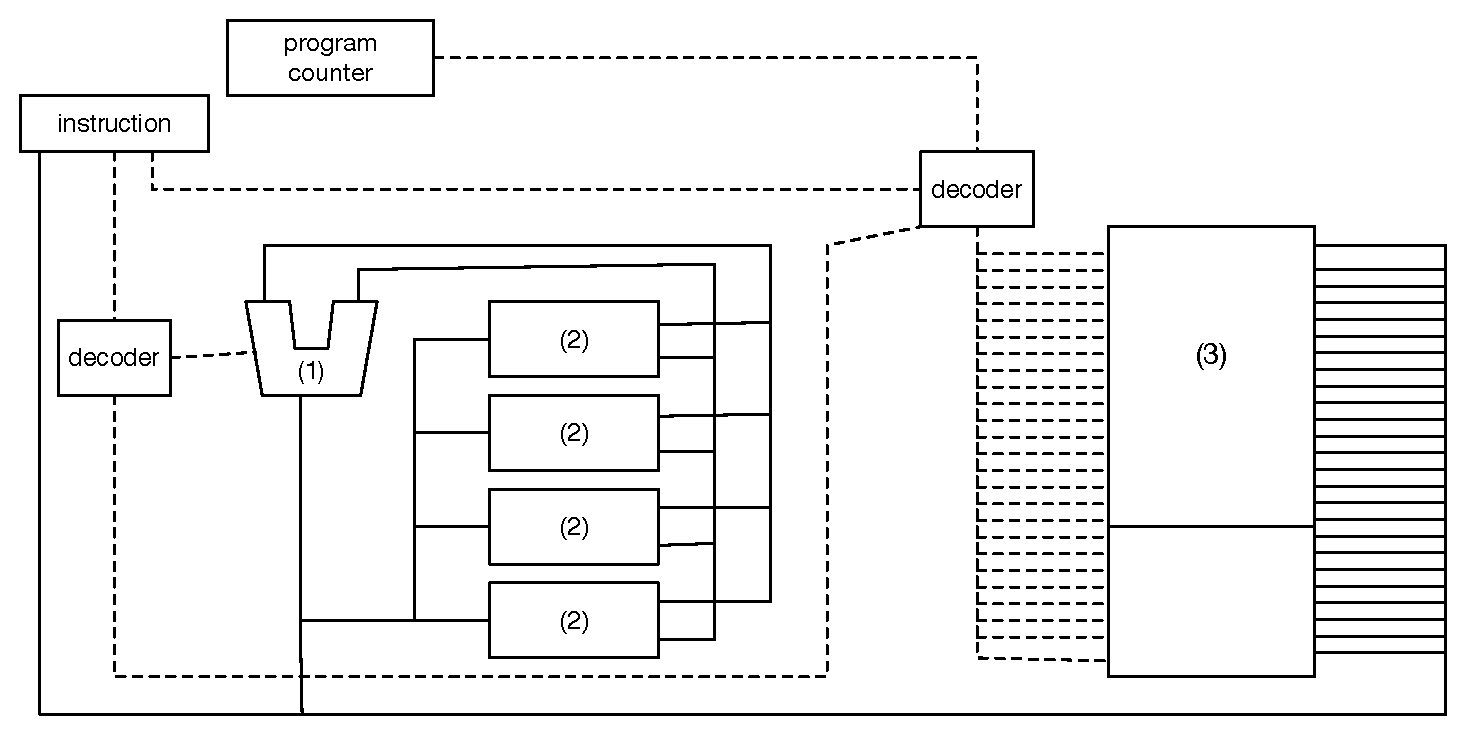
\includegraphics[scale=0.6]{./Figure/elementaryCS-figCPU-exam.eps}
  \end{center}

\hfill{裏面につづく}
\newpage

\paragraphskip
\nitem{\bf 問3.}(配点 10 点)\\
数学で考える関数と Ruby で出てくる関数
(講義や教科書ではサブルーチンと呼んでいた)
の違いを,対数関数 $\log_2(x)$ を例に説明せよ.

\paragraphskip
\nitem{\bf 問4.}(配点 15 点)\\
次に示したのは言語 Ruby で書かれたプログラムの一部
(サブルーチンの定義の部分)である.
このプログラムについて以下の問いに答えよ.

\begin{verbatim}
    def f(x, y)
    # assume: x > 0, y > 0
       res  = 1
       while y > 0
          if y % 2 == 1
             res = res * x
          end
          y = y / 2
          x = x * x
       end
       return res
    end
\end{verbatim}

\nitem{(1)}
このサブルーチンを用いて
{\tt f(2,2)}, {\tt f(2,3)}, {\tt f(2,9)}
を計算したときの値を示せ.
\nitem{(2)}
一般に,
正の自然数 $x,y$ に対して,
{\tt f(}$x$, $y${\tt)} は,
どのような関数を計算するかを述べよ.
\nitem{(3)}
{\tt f(3,1000)} の計算では,
while の繰り返しが何回行われるか?

\end{document}
